% Options for packages loaded elsewhere
\PassOptionsToPackage{unicode}{hyperref}
\PassOptionsToPackage{hyphens}{url}
%
\documentclass[
]{article}
\usepackage{lmodern}
\usepackage{amssymb,amsmath}
\usepackage{ifxetex,ifluatex}
\ifnum 0\ifxetex 1\fi\ifluatex 1\fi=0 % if pdftex
  \usepackage[T1]{fontenc}
  \usepackage[utf8]{inputenc}
  \usepackage{textcomp} % provide euro and other symbols
\else % if luatex or xetex
  \usepackage{unicode-math}
  \defaultfontfeatures{Scale=MatchLowercase}
  \defaultfontfeatures[\rmfamily]{Ligatures=TeX,Scale=1}
\fi
% Use upquote if available, for straight quotes in verbatim environments
\IfFileExists{upquote.sty}{\usepackage{upquote}}{}
\IfFileExists{microtype.sty}{% use microtype if available
  \usepackage[]{microtype}
  \UseMicrotypeSet[protrusion]{basicmath} % disable protrusion for tt fonts
}{}
\makeatletter
\@ifundefined{KOMAClassName}{% if non-KOMA class
  \IfFileExists{parskip.sty}{%
    \usepackage{parskip}
  }{% else
    \setlength{\parindent}{0pt}
    \setlength{\parskip}{6pt plus 2pt minus 1pt}}
}{% if KOMA class
  \KOMAoptions{parskip=half}}
\makeatother
\usepackage{xcolor}
\IfFileExists{xurl.sty}{\usepackage{xurl}}{} % add URL line breaks if available
\IfFileExists{bookmark.sty}{\usepackage{bookmark}}{\usepackage{hyperref}}
\hypersetup{
  pdftitle={Refugee Pop. 2019 - Climate Morality 2030 3D World Maps},
  pdfauthor={Maxwell Reikosky},
  hidelinks,
  pdfcreator={LaTeX via pandoc}}
\urlstyle{same} % disable monospaced font for URLs
\usepackage[margin=1in]{geometry}
\usepackage{color}
\usepackage{fancyvrb}
\newcommand{\VerbBar}{|}
\newcommand{\VERB}{\Verb[commandchars=\\\{\}]}
\DefineVerbatimEnvironment{Highlighting}{Verbatim}{commandchars=\\\{\}}
% Add ',fontsize=\small' for more characters per line
\usepackage{framed}
\definecolor{shadecolor}{RGB}{248,248,248}
\newenvironment{Shaded}{\begin{snugshade}}{\end{snugshade}}
\newcommand{\AlertTok}[1]{\textcolor[rgb]{0.94,0.16,0.16}{#1}}
\newcommand{\AnnotationTok}[1]{\textcolor[rgb]{0.56,0.35,0.01}{\textbf{\textit{#1}}}}
\newcommand{\AttributeTok}[1]{\textcolor[rgb]{0.77,0.63,0.00}{#1}}
\newcommand{\BaseNTok}[1]{\textcolor[rgb]{0.00,0.00,0.81}{#1}}
\newcommand{\BuiltInTok}[1]{#1}
\newcommand{\CharTok}[1]{\textcolor[rgb]{0.31,0.60,0.02}{#1}}
\newcommand{\CommentTok}[1]{\textcolor[rgb]{0.56,0.35,0.01}{\textit{#1}}}
\newcommand{\CommentVarTok}[1]{\textcolor[rgb]{0.56,0.35,0.01}{\textbf{\textit{#1}}}}
\newcommand{\ConstantTok}[1]{\textcolor[rgb]{0.00,0.00,0.00}{#1}}
\newcommand{\ControlFlowTok}[1]{\textcolor[rgb]{0.13,0.29,0.53}{\textbf{#1}}}
\newcommand{\DataTypeTok}[1]{\textcolor[rgb]{0.13,0.29,0.53}{#1}}
\newcommand{\DecValTok}[1]{\textcolor[rgb]{0.00,0.00,0.81}{#1}}
\newcommand{\DocumentationTok}[1]{\textcolor[rgb]{0.56,0.35,0.01}{\textbf{\textit{#1}}}}
\newcommand{\ErrorTok}[1]{\textcolor[rgb]{0.64,0.00,0.00}{\textbf{#1}}}
\newcommand{\ExtensionTok}[1]{#1}
\newcommand{\FloatTok}[1]{\textcolor[rgb]{0.00,0.00,0.81}{#1}}
\newcommand{\FunctionTok}[1]{\textcolor[rgb]{0.00,0.00,0.00}{#1}}
\newcommand{\ImportTok}[1]{#1}
\newcommand{\InformationTok}[1]{\textcolor[rgb]{0.56,0.35,0.01}{\textbf{\textit{#1}}}}
\newcommand{\KeywordTok}[1]{\textcolor[rgb]{0.13,0.29,0.53}{\textbf{#1}}}
\newcommand{\NormalTok}[1]{#1}
\newcommand{\OperatorTok}[1]{\textcolor[rgb]{0.81,0.36,0.00}{\textbf{#1}}}
\newcommand{\OtherTok}[1]{\textcolor[rgb]{0.56,0.35,0.01}{#1}}
\newcommand{\PreprocessorTok}[1]{\textcolor[rgb]{0.56,0.35,0.01}{\textit{#1}}}
\newcommand{\RegionMarkerTok}[1]{#1}
\newcommand{\SpecialCharTok}[1]{\textcolor[rgb]{0.00,0.00,0.00}{#1}}
\newcommand{\SpecialStringTok}[1]{\textcolor[rgb]{0.31,0.60,0.02}{#1}}
\newcommand{\StringTok}[1]{\textcolor[rgb]{0.31,0.60,0.02}{#1}}
\newcommand{\VariableTok}[1]{\textcolor[rgb]{0.00,0.00,0.00}{#1}}
\newcommand{\VerbatimStringTok}[1]{\textcolor[rgb]{0.31,0.60,0.02}{#1}}
\newcommand{\WarningTok}[1]{\textcolor[rgb]{0.56,0.35,0.01}{\textbf{\textit{#1}}}}
\usepackage{graphicx,grffile}
\makeatletter
\def\maxwidth{\ifdim\Gin@nat@width>\linewidth\linewidth\else\Gin@nat@width\fi}
\def\maxheight{\ifdim\Gin@nat@height>\textheight\textheight\else\Gin@nat@height\fi}
\makeatother
% Scale images if necessary, so that they will not overflow the page
% margins by default, and it is still possible to overwrite the defaults
% using explicit options in \includegraphics[width, height, ...]{}
\setkeys{Gin}{width=\maxwidth,height=\maxheight,keepaspectratio}
% Set default figure placement to htbp
\makeatletter
\def\fps@figure{htbp}
\makeatother
\setlength{\emergencystretch}{3em} % prevent overfull lines
\providecommand{\tightlist}{%
  \setlength{\itemsep}{0pt}\setlength{\parskip}{0pt}}
\setcounter{secnumdepth}{-\maxdimen} % remove section numbering

\title{Refugee Pop. 2019 - Climate Morality 2030 3D World Maps}
\author{Maxwell Reikosky}
\date{12/10/2020}

\begin{document}
\maketitle

\begin{Shaded}
\begin{Highlighting}[]
\CommentTok{# allowing r chunks to knit without printing 3D models that cause error}
\NormalTok{knitr}\OperatorTok{::}\NormalTok{opts_chunk}\OperatorTok{$}\KeywordTok{set}\NormalTok{(}\DataTypeTok{eval =}\NormalTok{ T)}
\end{Highlighting}
\end{Shaded}

\begin{Shaded}
\begin{Highlighting}[]
\KeywordTok{options}\NormalTok{(}\DataTypeTok{tinytex.verbose =} \OtherTok{TRUE}\NormalTok{)}
\end{Highlighting}
\end{Shaded}

\begin{Shaded}
\begin{Highlighting}[]
\CommentTok{# may need to run developer tools as administrator, commenting code below}
\CommentTok{# install.packages("devtools") }
\CommentTok{# devtools::install_github("tylermorganwall/rayshader")}

\CommentTok{# loading relevant packages}
\KeywordTok{library}\NormalTok{(readxl)}
\KeywordTok{library}\NormalTok{(dplyr)}
\KeywordTok{library}\NormalTok{(ggplot2)}
\KeywordTok{library}\NormalTok{(ggmap)}
\KeywordTok{library}\NormalTok{(rayshader)}
\KeywordTok{library}\NormalTok{(tidyverse)}
\KeywordTok{library}\NormalTok{(rlang)}
\KeywordTok{library}\NormalTok{(rgl)}
\KeywordTok{require}\NormalTok{(devtools)}
\KeywordTok{library}\NormalTok{(tinytex)}


\KeywordTok{rgl.open}\NormalTok{()}
\end{Highlighting}
\end{Shaded}

\hypertarget{importing-and-cleaning-refugee-pop.-dataset}{%
\subsection{1. Importing and Cleaning Refugee Pop.
Dataset}\label{importing-and-cleaning-refugee-pop.-dataset}}

\begin{Shaded}
\begin{Highlighting}[]
\CommentTok{# must set working directory to MaxwellReikosky_CompToolsFinal folder}
\CommentTok{# loading refugee population by country of asylum dataset}
\NormalTok{Refugee_totals <-}\StringTok{ }\KeywordTok{read_excel}\NormalTok{(}\StringTok{"Data/WORLD BANKAPI_SM.POP.REFG_DS2_en_excel_v2_1743495.xls"}\NormalTok{)}

\CommentTok{# renaming relevant column as a workable string}
\NormalTok{Refugee_totals <-}\StringTok{ }\NormalTok{Refugee_totals }\OperatorTok
\StringTok{  }\KeywordTok{rename}\NormalTok{(}\StringTok{"year_2019"}\NormalTok{ =}\StringTok{ "2019"}\NormalTok{)}
  
\CommentTok{# subsetting refugee dataset to most recent measurement }
\NormalTok{Refugee_totals <-}\StringTok{ }\NormalTok{Refugee_totals }\OperatorTok
\StringTok{  }\KeywordTok{select}\NormalTok{(Country_name, year_}\DecValTok{2019}\NormalTok{) }\OperatorTok

\CommentTok{# trimming white space}
\StringTok{  }\KeywordTok{mutate}\NormalTok{(}\DataTypeTok{Country_name =} \KeywordTok{str_trim}\NormalTok{(Country_name), }
         \DataTypeTok{year_2019 =} \KeywordTok{str_trim}\NormalTok{(year_}\DecValTok{2019}\NormalTok{)) }\OperatorTok
\StringTok{  }
\CommentTok{# omitting all countries that were not measured}
\StringTok{  }\KeywordTok{na.omit}\NormalTok{()}

\CommentTok{# recoding country names to match map.world df}
\CommentTok{# needed escape symbol for recoding Cote d'Ivoire }
\NormalTok{Refugee_totals}\OperatorTok{$}\NormalTok{Country_name <-}\StringTok{ }\KeywordTok{recode}\NormalTok{(Refugee_totals}\OperatorTok{$}\NormalTok{Country_name, }
                                      \StringTok{'United States'}\NormalTok{ =}\StringTok{ 'USA'}\NormalTok{,}
                                      \StringTok{'United Kingdom'}\NormalTok{ =}\StringTok{ 'UK'}\NormalTok{, }
                                      \StringTok{'Russian Federation'}\NormalTok{ =}\StringTok{ 'Russia'}\NormalTok{, }
                                      \StringTok{'Congo, Dem. Rep.'}\NormalTok{ =}\StringTok{ 'Democratic Republic of the Congo'}\NormalTok{,}
                                      \StringTok{'Congo, Rep.'}\NormalTok{ =}\StringTok{ 'Republic of Congo'}\NormalTok{, }
                                      \StringTok{'Korea, Rep.'}\NormalTok{ =}\StringTok{ 'North Korea'}\NormalTok{, }
                                      \StringTok{'Cote d}\CharTok{\textbackslash{}'}\StringTok{Ivoire'}\NormalTok{ =}\StringTok{ 'Ivory Coast'}\NormalTok{, }
                                      \StringTok{'Egypt, Arab Rep.'}\NormalTok{ =}\StringTok{ 'Egypt'}\NormalTok{, }
                                      \StringTok{'Venezuela, RB'}\NormalTok{ =}\StringTok{ 'Venezuela'}\NormalTok{, }
                                      \StringTok{'Yemen, Rep.'}\NormalTok{ =}\StringTok{ 'Yemen'}\NormalTok{, }
                                      \StringTok{'Syrian Arab Republic'}\NormalTok{ =}\StringTok{ 'Syria'}\NormalTok{, }
                                      \StringTok{'Slovak Republic'}\NormalTok{ =}\StringTok{ 'Slovakia'}\NormalTok{, }
                                      \StringTok{'Kyrgyz Republic'}\NormalTok{ =}\StringTok{ 'Kyrgyzstan'}\NormalTok{, }
                                      \StringTok{'North Macedonia'}\NormalTok{ =}\StringTok{ 'Macedonia'}\NormalTok{, }
                                      \StringTok{'Bahamas, The'}\NormalTok{ =}\StringTok{ 'Bahamas'}\NormalTok{, }
                                      \StringTok{'Gambia, The'}\NormalTok{ =}\StringTok{ 'Gambia'}\NormalTok{, }
                                      \StringTok{'Iran, Islamic Rep.'}\NormalTok{ =}\StringTok{ 'Iran'}\NormalTok{, }
                                      \StringTok{'West Bank and Gaza'}\NormalTok{ =}\StringTok{ 'Gaza Strip'}\NormalTok{)}
\end{Highlighting}
\end{Shaded}

\hypertarget{importing-world-map-dataset}{%
\subsection{2. Importing World Map
Dataset}\label{importing-world-map-dataset}}

\begin{Shaded}
\begin{Highlighting}[]
\CommentTok{# grabbing world map df}
\NormalTok{map.world <-}\StringTok{ }\KeywordTok{map_data}\NormalTok{(}\StringTok{"world"}\NormalTok{)}

\CommentTok{# checking how many countries are listed on world map dataset}
\NormalTok{map.world }\OperatorTok
\KeywordTok{select}\NormalTok{(region) }\OperatorTok
\KeywordTok{unique}\NormalTok{()}
\end{Highlighting}
\end{Shaded}

\hypertarget{joining-world-map-and-refugee-pop.-datasets}{%
\subsection{3. Joining World Map and Refugee Pop.
Datasets}\label{joining-world-map-and-refugee-pop.-datasets}}

\begin{Shaded}
\begin{Highlighting}[]
\CommentTok{# merging map and recoded refugee pop datasets}
\NormalTok{Refugee_map <-}\StringTok{ }\KeywordTok{left_join}\NormalTok{(map.world, Refugee_totals, }\DataTypeTok{by =} \KeywordTok{c}\NormalTok{(}\StringTok{'region'}\NormalTok{ =}\StringTok{ 'Country_name'}\NormalTok{))}

\CommentTok{# converting year_2019 to numeric because some were in character type}
\NormalTok{Refugee_map}\OperatorTok{$}\NormalTok{year_}\DecValTok{2019}\NormalTok{ <-}\StringTok{ }\KeywordTok{as.numeric}\NormalTok{(Refugee_map}\OperatorTok{$}\NormalTok{year_}\DecValTok{2019}\NormalTok{)}
\end{Highlighting}
\end{Shaded}

\hypertarget{importing-and-cleaning-climate-vulnerability-dataset}{%
\subsection{4. Importing and Cleaning Climate Vulnerability
Dataset}\label{importing-and-cleaning-climate-vulnerability-dataset}}

\begin{Shaded}
\begin{Highlighting}[]
\CommentTok{# loading climate vulnerability excel data set}
\NormalTok{Climate_totals <-}\StringTok{ }\KeywordTok{read_excel}\NormalTok{(}\StringTok{"Data/Climate_totals.xls"}\NormalTok{)}

\CommentTok{# Renaming climate mortality column to workable string}
\NormalTok{Climate_totals <-}\StringTok{ }\NormalTok{Climate_totals }\OperatorTok
\StringTok{  }\KeywordTok{rename}\NormalTok{(}\StringTok{"Climate_mortality"}\NormalTok{ =}\StringTok{ "Mortality_Climate_total_2030 (Number of People)"}\NormalTok{)}

\CommentTok{# recoding country names to fit map.world dataset}
\NormalTok{Climate_totals}\OperatorTok{$}\NormalTok{Country_name <-}\StringTok{ }\KeywordTok{recode}\NormalTok{(Climate_totals}\OperatorTok{$}\NormalTok{Country_name, }
                                      \StringTok{'United States'}\NormalTok{ =}\StringTok{ 'USA'}\NormalTok{, }
                                      \StringTok{'United Kingdom'}\NormalTok{ =}\StringTok{ 'UK'}\NormalTok{, }
                                      \StringTok{'Congo'}\NormalTok{ =}\StringTok{ 'Republic of Congo'}\NormalTok{, }
                                      \StringTok{'Cote d}\CharTok{\textbackslash{}'}\StringTok{Ivoire'}\NormalTok{ =}\StringTok{ 'Ivory Coast'}\NormalTok{, }
                                      \StringTok{'DR Congo'}\NormalTok{ =}\StringTok{ 'Democratic Republic of the Congo'}\NormalTok{, }
                                      \StringTok{'Sudan/South Sudan1'}\NormalTok{ =}\StringTok{ 'South Sudan'}\NormalTok{, }
                                      \StringTok{'Sudan/South Sudan2'}\NormalTok{ =}\StringTok{ 'Sudan'}\NormalTok{)}

\CommentTok{# subsetting to select only 2030 climate mortality column}
\CommentTok{# clearing any potential white space}
\NormalTok{Climate_totals <-}\StringTok{ }\NormalTok{Climate_totals }\OperatorTok
\StringTok{  }\KeywordTok{select}\NormalTok{(Country_name, Climate_mortality) }\OperatorTok
\StringTok{  }\KeywordTok{mutate}\NormalTok{(}\DataTypeTok{Country_name =} \KeywordTok{str_trim}\NormalTok{(Country_name), }
         \DataTypeTok{Climate_mortality =} \KeywordTok{str_trim}\NormalTok{(Climate_mortality))}
\end{Highlighting}
\end{Shaded}

\hypertarget{joining-climate-mortality-with-previous-merged-dataset}{%
\subsection{5. Joining Climate Mortality With Previous Merged
Dataset}\label{joining-climate-mortality-with-previous-merged-dataset}}

\begin{Shaded}
\begin{Highlighting}[]
\CommentTok{# merging trimmed climate mortality dataset with previously merged dataset}
\NormalTok{Refclim_mapdf <-}\StringTok{ }\KeywordTok{left_join}\NormalTok{(Refugee_map, Climate_totals, }\DataTypeTok{by =} \KeywordTok{c}\NormalTok{(}\StringTok{'region'}\NormalTok{ =}\StringTok{ 'Country_name'}\NormalTok{))}

\CommentTok{# coercing climate mortality data to numerical because some were characters}
\NormalTok{Refclim_mapdf}\OperatorTok{$}\NormalTok{Climate_mortality <-}\StringTok{ }\KeywordTok{as.numeric}\NormalTok{(Refclim_mapdf}\OperatorTok{$}\NormalTok{Climate_mortality)}
\end{Highlighting}
\end{Shaded}

\hypertarget{refugee-population-by-country-2019-3d-model}{%
\subsection{6. Refugee Population by Country 2019 3D
Model}\label{refugee-population-by-country-2019-3d-model}}

\begin{Shaded}
\begin{Highlighting}[]
\CommentTok{# plotting refugee population by country}
\NormalTok{refpop_gg <-}\StringTok{ }\KeywordTok{ggplot}\NormalTok{(Refugee_map, }\KeywordTok{aes}\NormalTok{(long, lat, }\DataTypeTok{group =}\NormalTok{ group, }\DataTypeTok{fill =}\NormalTok{ year_}\DecValTok{2019}\NormalTok{)) }\OperatorTok{+}\StringTok{ }
\StringTok{  }
\CommentTok{# allowing flexible plot shape to match country borders}
\StringTok{  }\KeywordTok{geom_polygon}\NormalTok{() }\OperatorTok{+}\StringTok{ }

\CommentTok{# coloring countries on a chosen gradient for value range}
\StringTok{  }\KeywordTok{scale_fill_gradient}\NormalTok{(}\DataTypeTok{low =} \StringTok{"seashell"}\NormalTok{, }\DataTypeTok{high =} \StringTok{"darkgreen"}\NormalTok{) }\OperatorTok{+}\StringTok{ }
\StringTok{ }
\CommentTok{# labeling title and x & y axes}
\StringTok{  }\KeywordTok{labs}\NormalTok{(}\DataTypeTok{title =} \StringTok{"Refugee Pop. 2019"}\NormalTok{) }\OperatorTok{+}\StringTok{ }
\StringTok{  }\KeywordTok{xlab}\NormalTok{(}\StringTok{"Long."}\NormalTok{) }\OperatorTok{+}\StringTok{ }
\StringTok{  }\KeywordTok{ylab}\NormalTok{(}\StringTok{"Lat."}\NormalTok{) }\OperatorTok{+}\StringTok{ }
\StringTok{ }
\CommentTok{# removing legend title and setting background type}
\StringTok{   }\KeywordTok{theme}\NormalTok{(}\DataTypeTok{legend.title =} \KeywordTok{element_blank}\NormalTok{(), }
        \DataTypeTok{panel.background =} \KeywordTok{element_rect}\NormalTok{())}

\CommentTok{# rendering ggplot as 3D in rayshader, setting parameters and scale}
\KeywordTok{plot_gg}\NormalTok{(refpop_gg, }\DataTypeTok{width =} \DecValTok{5}\NormalTok{, }\DataTypeTok{height =} \DecValTok{5}\NormalTok{, }\DataTypeTok{raytrace =} \OtherTok{FALSE}\NormalTok{, }\DataTypeTok{preview =} \OtherTok{TRUE}\NormalTok{) }\OperatorTok{+}\StringTok{ }
\StringTok{  }\KeywordTok{plot_gg}\NormalTok{(refpop_gg , }\DataTypeTok{width =} \DecValTok{5}\NormalTok{, }\DataTypeTok{height =} \DecValTok{5}\NormalTok{, }\DataTypeTok{multicore =} \OtherTok{TRUE}\NormalTok{, }\DataTypeTok{scale =} \DecValTok{250}\NormalTok{,}
                                                                                      
\CommentTok{# establishing tilt of model and angle of snapshot perspective}
        \DataTypeTok{zoom =} \FloatTok{0.5}\NormalTok{, }\DataTypeTok{theta =} \DecValTok{7}\NormalTok{, }\DataTypeTok{phi =} \DecValTok{35}\NormalTok{, }\DataTypeTok{windowsize =} \KeywordTok{c}\NormalTok{(}\DecValTok{1200}\NormalTok{, }\DecValTok{800}\NormalTok{)) }\OperatorTok{+}\StringTok{ }
\StringTok{  }
\CommentTok{# allowing process launched from R to read input files before execution resumes}
\StringTok{  }\KeywordTok{Sys.sleep}\NormalTok{(}\FloatTok{0.2}\NormalTok{) }\OperatorTok{+}\StringTok{ }
\StringTok{  }
\CommentTok{# constructing snapshot of final 3D model}
\StringTok{  }\KeywordTok{render_snapshot}\NormalTok{(}\DataTypeTok{clear =} \OtherTok{TRUE}\NormalTok{) }
\end{Highlighting}
\end{Shaded}

\includegraphics{MaxwellReikosky_CompToolsFinal_files/figure-latex/unnamed-chunk-8-1.pdf}
\includegraphics{MaxwellReikosky_CompToolsFinal_files/figure-latex/unnamed-chunk-8-2.pdf}

\begin{Shaded}
\begin{Highlighting}[]
\KeywordTok{rglwidget}\NormalTok{()}
\end{Highlighting}
\end{Shaded}

\includegraphics[width=6.5in]{C:\Users\mreik\AppData\Local\Temp\RtmpMnKS65\file503c99579e0}

\begin{figure}
\centering
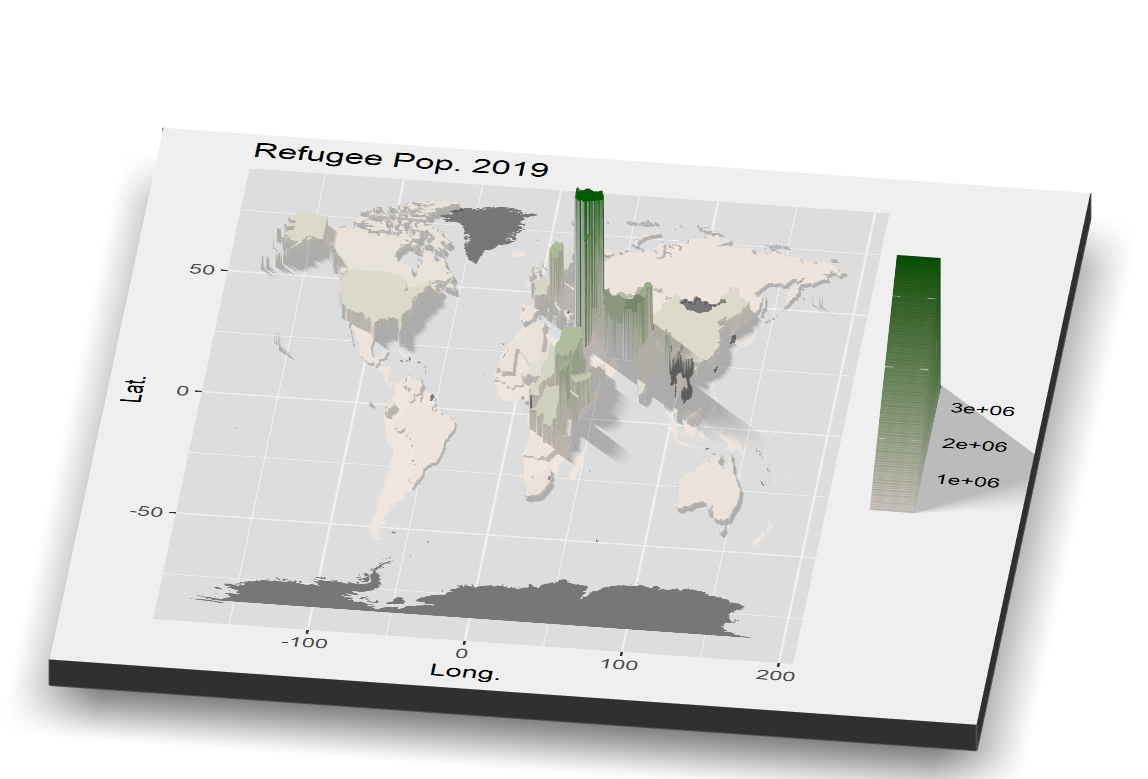
\includegraphics{Results/refpop.png}
\caption{``Refugee Population by Country 2019''}
\end{figure}

\hypertarget{refugee-population-by-country-2019-3d-model-sans-turkey-jordan}{%
\subsection{7. Refugee Population by Country 2019 3D Model (sans Turkey
\&
Jordan)}\label{refugee-population-by-country-2019-3d-model-sans-turkey-jordan}}

\begin{Shaded}
\begin{Highlighting}[]
\KeywordTok{rgl.close}\NormalTok{()}

\KeywordTok{rgl.open}\NormalTok{()}

\CommentTok{# filtering Turkey and Jordan to highlight other standout countries}
\NormalTok{refpop_sans <-}\StringTok{ }\NormalTok{Refugee_map }\OperatorTok
\StringTok{  }\KeywordTok{filter}\NormalTok{(region }\OperatorTok{!=}\StringTok{ "Turkey"}\NormalTok{,}
\NormalTok{         region }\OperatorTok{!=}\StringTok{ "Jordan"}\NormalTok{)}

\CommentTok{# plotting refugee population by country without Turkey and Jordan}
\NormalTok{refpop_sansgg <-}\StringTok{ }\KeywordTok{ggplot}\NormalTok{(refpop_sans, }\KeywordTok{aes}\NormalTok{(long, lat, }\DataTypeTok{group =}\NormalTok{ group, }\DataTypeTok{fill =}\NormalTok{ year_}\DecValTok{2019}\NormalTok{)) }\OperatorTok{+}\StringTok{ }
\StringTok{  }
\CommentTok{# allowing flexible plot shape to match country borders}
\StringTok{  }\KeywordTok{geom_polygon}\NormalTok{() }\OperatorTok{+}\StringTok{ }
\StringTok{  }
\CommentTok{# coloring countries on a chosen gradient for value range}
\StringTok{  }\KeywordTok{scale_fill_gradient}\NormalTok{(}\DataTypeTok{low =} \StringTok{"seashell"}\NormalTok{, }\DataTypeTok{high =} \StringTok{"darkgreen"}\NormalTok{) }\OperatorTok{+}\StringTok{ }
\StringTok{  }
\CommentTok{# labeling title and x & y axes}
\StringTok{  }\KeywordTok{labs}\NormalTok{(}\DataTypeTok{title =} \StringTok{"Refugee Pop. 2019 (sans Turkey & Jordan"}\NormalTok{) }\OperatorTok{+}\StringTok{ }
\StringTok{  }\KeywordTok{xlab}\NormalTok{(}\StringTok{"Long."}\NormalTok{) }\OperatorTok{+}\StringTok{ }
\StringTok{  }\KeywordTok{ylab}\NormalTok{(}\StringTok{"Lat."}\NormalTok{) }\OperatorTok{+}\StringTok{ }
\StringTok{  }
\CommentTok{# removing legend title and setting background type}
\StringTok{  }\KeywordTok{theme}\NormalTok{(}\DataTypeTok{legend.title =} \KeywordTok{element_blank}\NormalTok{(),}
        \DataTypeTok{panel.background =} \KeywordTok{element_rect}\NormalTok{())}


\CommentTok{# rendering ggplot as 3D in rayshader, setting parameters and scale}
\KeywordTok{plot_gg}\NormalTok{(refpop_sansgg, }\DataTypeTok{width =} \DecValTok{5}\NormalTok{, }\DataTypeTok{height =} \DecValTok{5}\NormalTok{, }\DataTypeTok{raytrace =} \OtherTok{FALSE}\NormalTok{, }\DataTypeTok{preview =} \OtherTok{TRUE}\NormalTok{) }\OperatorTok{+}\StringTok{ }
\KeywordTok{plot_gg}\NormalTok{(refpop_sansgg, }\DataTypeTok{width =} \DecValTok{5}\NormalTok{, }\DataTypeTok{height =} \DecValTok{5}\NormalTok{, }\DataTypeTok{multicore =} \OtherTok{TRUE}\NormalTok{, }\DataTypeTok{scale =} \DecValTok{250}\NormalTok{,}
        
\CommentTok{# establishing angle of snapshot perspective}
        \DataTypeTok{zoom =} \FloatTok{0.5}\NormalTok{, }\DataTypeTok{theta =} \DecValTok{7}\NormalTok{, }\DataTypeTok{phi =} \DecValTok{35}\NormalTok{, }\DataTypeTok{windowsize =} \KeywordTok{c}\NormalTok{(}\DecValTok{1200}\NormalTok{, }\DecValTok{800}\NormalTok{)) }\OperatorTok{+}\StringTok{ }
\StringTok{  }
\CommentTok{# allowing process launched from R to read input files before execution resumes}
\StringTok{  }\KeywordTok{Sys.sleep}\NormalTok{(}\FloatTok{0.2}\NormalTok{) }\OperatorTok{+}\StringTok{ }
\StringTok{  }
\CommentTok{# constructing snapshot of final 3D model}
\StringTok{  }\KeywordTok{render_snapshot}\NormalTok{(}\DataTypeTok{clear =} \OtherTok{TRUE}\NormalTok{) }
\end{Highlighting}
\end{Shaded}

\includegraphics{MaxwellReikosky_CompToolsFinal_files/figure-latex/unnamed-chunk-9-1.pdf}
\includegraphics{MaxwellReikosky_CompToolsFinal_files/figure-latex/unnamed-chunk-9-2.pdf}

\begin{Shaded}
\begin{Highlighting}[]
\KeywordTok{rglwidget}\NormalTok{()}
\end{Highlighting}
\end{Shaded}

\includegraphics[width=6.5in]{C:\Users\mreik\AppData\Local\Temp\RtmpMnKS65\file503c3fef19f7}

\newpage

\begin{figure}
\centering
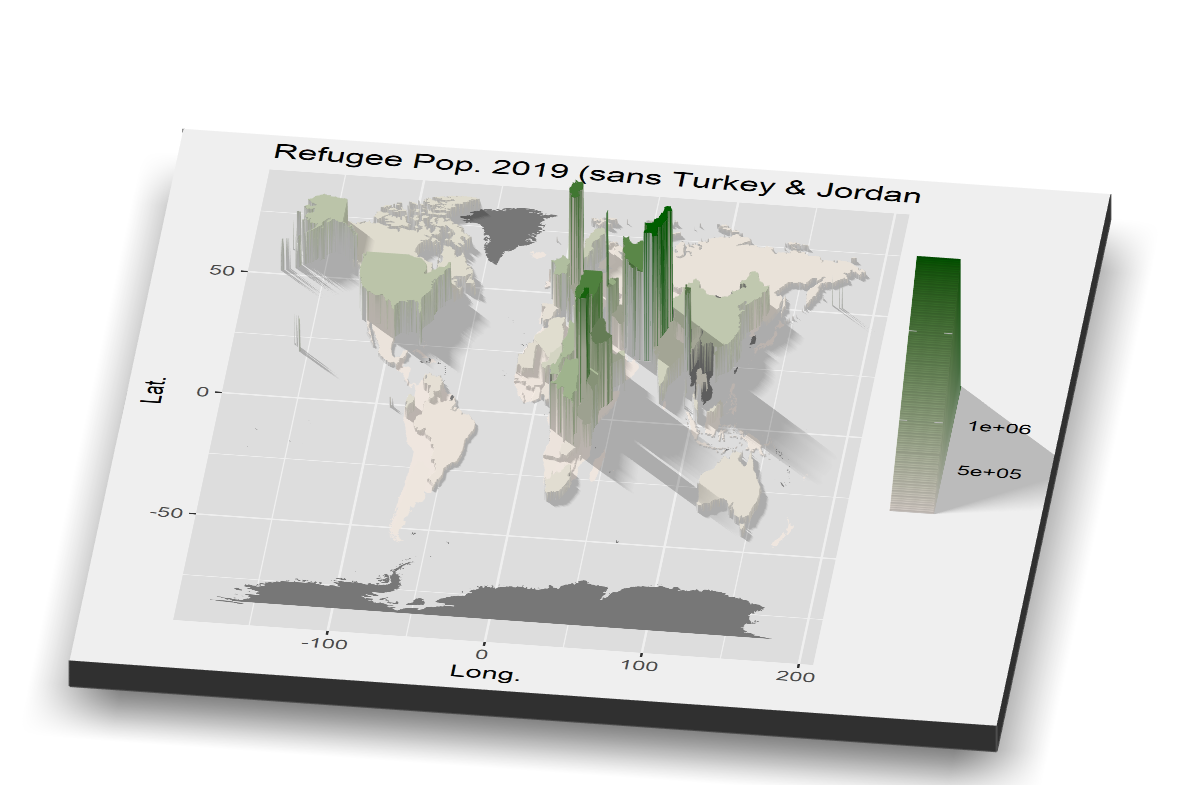
\includegraphics{Results/refpop_sansturjor.png}
\caption{``Refugee Population by Country 2019 (sans Turkey \& Jordan)''}
\end{figure}

\newpage

\hypertarget{climate-mortality-2030-by-country-3d-model}{%
\subsection{8. Climate Mortality 2030 by Country 3D
Model}\label{climate-mortality-2030-by-country-3d-model}}

\begin{Shaded}
\begin{Highlighting}[]
\CommentTok{# plotting climate mortality in 2030 by country }
\NormalTok{climmort_gg <-}\StringTok{ }\KeywordTok{ggplot}\NormalTok{(Refclim_mapdf, }\KeywordTok{aes}\NormalTok{(long, lat, }\DataTypeTok{group =}\NormalTok{ group, }\DataTypeTok{fill =}\NormalTok{ Climate_mortality)) }\OperatorTok{+}\StringTok{ }

\CommentTok{# allowing flexible shape to match country borders}
\StringTok{  }\KeywordTok{geom_polygon}\NormalTok{() }\OperatorTok{+}\StringTok{ }
\StringTok{  }
\CommentTok{# coloring countries on a chosen gradient for value range}
\StringTok{  }\KeywordTok{scale_fill_gradient}\NormalTok{(}\DataTypeTok{low =} \StringTok{"seashell"}\NormalTok{, }\DataTypeTok{high =} \StringTok{"darkred"}\NormalTok{) }\OperatorTok{+}\StringTok{ }
\StringTok{  }
\CommentTok{# labeling title and x & y axes}
\StringTok{  }\KeywordTok{labs}\NormalTok{(}\DataTypeTok{title =} \StringTok{"Climate Mortality 2030"}\NormalTok{) }\OperatorTok{+}\StringTok{ }
\StringTok{  }\KeywordTok{theme}\NormalTok{() }\OperatorTok{+}\StringTok{ }
\StringTok{  }\KeywordTok{xlab}\NormalTok{(}\StringTok{"Long."}\NormalTok{) }\OperatorTok{+}\StringTok{ }
\StringTok{  }\KeywordTok{ylab}\NormalTok{(}\StringTok{"Lat."}\NormalTok{) }\OperatorTok{+}\StringTok{ }
\StringTok{ }
\CommentTok{# removing legend title and setting background type}
\StringTok{  }\KeywordTok{theme}\NormalTok{(}\DataTypeTok{legend.title =} \KeywordTok{element_blank}\NormalTok{(), }
         \DataTypeTok{panel.background =} \KeywordTok{element_rect}\NormalTok{())}


\CommentTok{# rendering ggplot as 3D in rayshader, setting parameters and scale}
\KeywordTok{plot_gg}\NormalTok{(climmort_gg, }\DataTypeTok{width =} \DecValTok{5}\NormalTok{, }\DataTypeTok{height =} \DecValTok{5}\NormalTok{, }\DataTypeTok{raytrace =} \OtherTok{FALSE}\NormalTok{, }\DataTypeTok{preview =} \OtherTok{TRUE}\NormalTok{) }\OperatorTok{+}\StringTok{ }
\StringTok{  }\KeywordTok{plot_gg}\NormalTok{(climmort_gg, }\DataTypeTok{width =} \DecValTok{5}\NormalTok{, }\DataTypeTok{height =} \DecValTok{5}\NormalTok{, }\DataTypeTok{multicore =} \OtherTok{TRUE}\NormalTok{, }\DataTypeTok{scale =} \DecValTok{250}\NormalTok{, }
                                                                                       
\CommentTok{# establishing angle of snapshot perspective                                           }
    \DataTypeTok{zoom =} \FloatTok{0.5}\NormalTok{, }\DataTypeTok{theta =} \DecValTok{7}\NormalTok{, }\DataTypeTok{phi =} \DecValTok{35}\NormalTok{, }\DataTypeTok{windowsize =} \KeywordTok{c}\NormalTok{(}\DecValTok{1200}\NormalTok{, }\DecValTok{800}\NormalTok{)) }\OperatorTok{+}\StringTok{ }
\StringTok{  }
\CommentTok{# allowing process launched from R to read input files before execution resumes}
\StringTok{  }\KeywordTok{Sys.sleep}\NormalTok{(}\FloatTok{0.2}\NormalTok{) }\OperatorTok{+}\StringTok{ }
\StringTok{  }
\CommentTok{# constructing snapshot of final 3D model}
\StringTok{  }\KeywordTok{render_snapshot}\NormalTok{(}\DataTypeTok{clear =} \OtherTok{TRUE}\NormalTok{) }
\end{Highlighting}
\end{Shaded}

\includegraphics{MaxwellReikosky_CompToolsFinal_files/figure-latex/unnamed-chunk-10-1.pdf}
\includegraphics{MaxwellReikosky_CompToolsFinal_files/figure-latex/unnamed-chunk-10-2.pdf}

\newpage

\begin{figure}
\centering
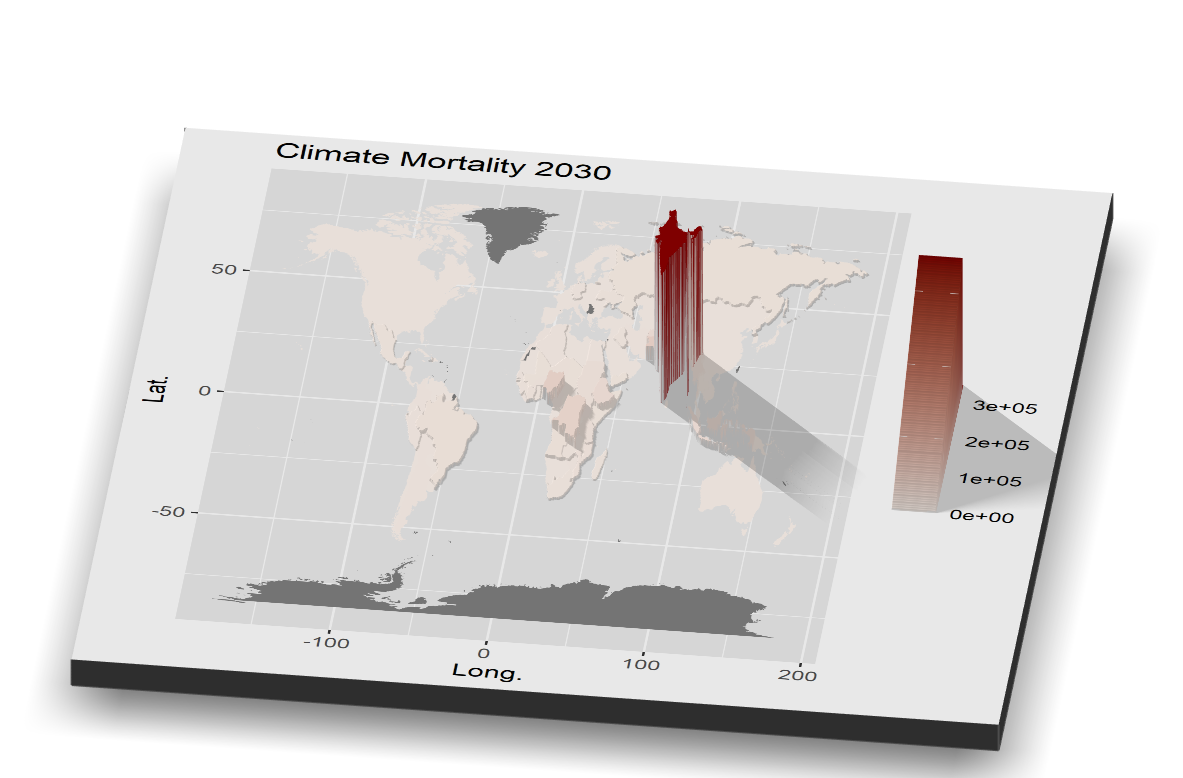
\includegraphics{Results/climmort.png}
\caption{``Climate Mortality 2030 by Country''}
\end{figure}

\newpage

\hypertarget{climate-mortality-2030-by-country-3d-model-sans-india}{%
\subsection{9. Climate Mortality 2030 by Country 3D Model (sans
India)}\label{climate-mortality-2030-by-country-3d-model-sans-india}}

\begin{Shaded}
\begin{Highlighting}[]
\CommentTok{# filtering out India to calibrate for its disproportionate mortality}
\NormalTok{climmort_sans <-}\StringTok{ }\NormalTok{Refclim_mapdf }\OperatorTok
\StringTok{  }\KeywordTok{filter}\NormalTok{(region }\OperatorTok{!=}\StringTok{ "India"}\NormalTok{)}

\CommentTok{# plotting climate mortality in 2030 by country, excluding India}
\NormalTok{climmort_sansgg <-}\StringTok{ }\KeywordTok{ggplot}\NormalTok{(climmort_sans, }\KeywordTok{aes}\NormalTok{(long, lat, }\DataTypeTok{group =}\NormalTok{ group, }\DataTypeTok{fill =}\NormalTok{ Climate_mortality)) }\OperatorTok{+}\StringTok{ }
\StringTok{  }
\CommentTok{# allowing flexible plot shape to match country borders}
\StringTok{  }\KeywordTok{geom_polygon}\NormalTok{() }\OperatorTok{+}\StringTok{ }
\StringTok{  }
\CommentTok{# coloring countries on a chosen gradient for value range}
\StringTok{  }\KeywordTok{scale_fill_gradient}\NormalTok{(}\DataTypeTok{low =} \StringTok{"seashell"}\NormalTok{, }\DataTypeTok{high =} \StringTok{"darkred"}\NormalTok{) }\OperatorTok{+}\StringTok{ }
\StringTok{  }
\CommentTok{# labeling title and x & y axes}
\StringTok{  }\KeywordTok{labs}\NormalTok{(}\DataTypeTok{title =} \StringTok{"Climate Mortality 2030 (sans India)"}\NormalTok{) }\OperatorTok{+}\StringTok{ }
\StringTok{  }\KeywordTok{xlab}\NormalTok{(}\StringTok{"Long."}\NormalTok{) }\OperatorTok{+}\StringTok{ }
\StringTok{  }\KeywordTok{ylab}\NormalTok{(}\StringTok{"Lat."}\NormalTok{) }\OperatorTok{+}\StringTok{ }
\StringTok{  }
\CommentTok{# removing legend title and setting background type}
\StringTok{  }\KeywordTok{theme}\NormalTok{(}\DataTypeTok{legend.title =} \KeywordTok{element_blank}\NormalTok{(),}
        \DataTypeTok{panel.background =} \KeywordTok{element_rect}\NormalTok{())}

\CommentTok{# rendering ggplot as 3D in rayshader, setting parameters and scale}
\KeywordTok{plot_gg}\NormalTok{(climmort_sansgg, }\DataTypeTok{width =} \DecValTok{5}\NormalTok{, }\DataTypeTok{height =} \DecValTok{5}\NormalTok{, }\DataTypeTok{raytrace =} \OtherTok{FALSE}\NormalTok{, }\DataTypeTok{preview =} \OtherTok{TRUE}\NormalTok{) }\OperatorTok{+}
\StringTok{  }\KeywordTok{plot_gg}\NormalTok{(climmort_sansgg, }\DataTypeTok{width =} \DecValTok{5}\NormalTok{, }\DataTypeTok{height =} \DecValTok{5}\NormalTok{, }\DataTypeTok{multicore =} \OtherTok{TRUE}\NormalTok{, }\DataTypeTok{scale =} \DecValTok{250}\NormalTok{,}
                                                                                           
\CommentTok{# establishing angle of snapshot perspective }
    \DataTypeTok{zoom =} \FloatTok{0.5}\NormalTok{, }\DataTypeTok{theta =} \DecValTok{7}\NormalTok{, }\DataTypeTok{phi =} \DecValTok{35}\NormalTok{, }\DataTypeTok{windowsize =} \KeywordTok{c}\NormalTok{(}\DecValTok{1200}\NormalTok{, }\DecValTok{800}\NormalTok{)) }\OperatorTok{+}\StringTok{ }
\StringTok{  }
\CommentTok{# allowing process launched from R to read input files before execution resumes}
\StringTok{  }\KeywordTok{Sys.sleep}\NormalTok{(}\FloatTok{0.2}\NormalTok{) }\OperatorTok{+}\StringTok{ }

\CommentTok{# constructing snapshot of final 3D model }
\StringTok{  }\KeywordTok{render_snapshot}\NormalTok{(}\DataTypeTok{clear =} \OtherTok{TRUE}\NormalTok{)}
\end{Highlighting}
\end{Shaded}

\includegraphics{MaxwellReikosky_CompToolsFinal_files/figure-latex/unnamed-chunk-11-1.pdf}
\includegraphics{MaxwellReikosky_CompToolsFinal_files/figure-latex/unnamed-chunk-11-2.pdf}

\newpage

\begin{figure}
\centering
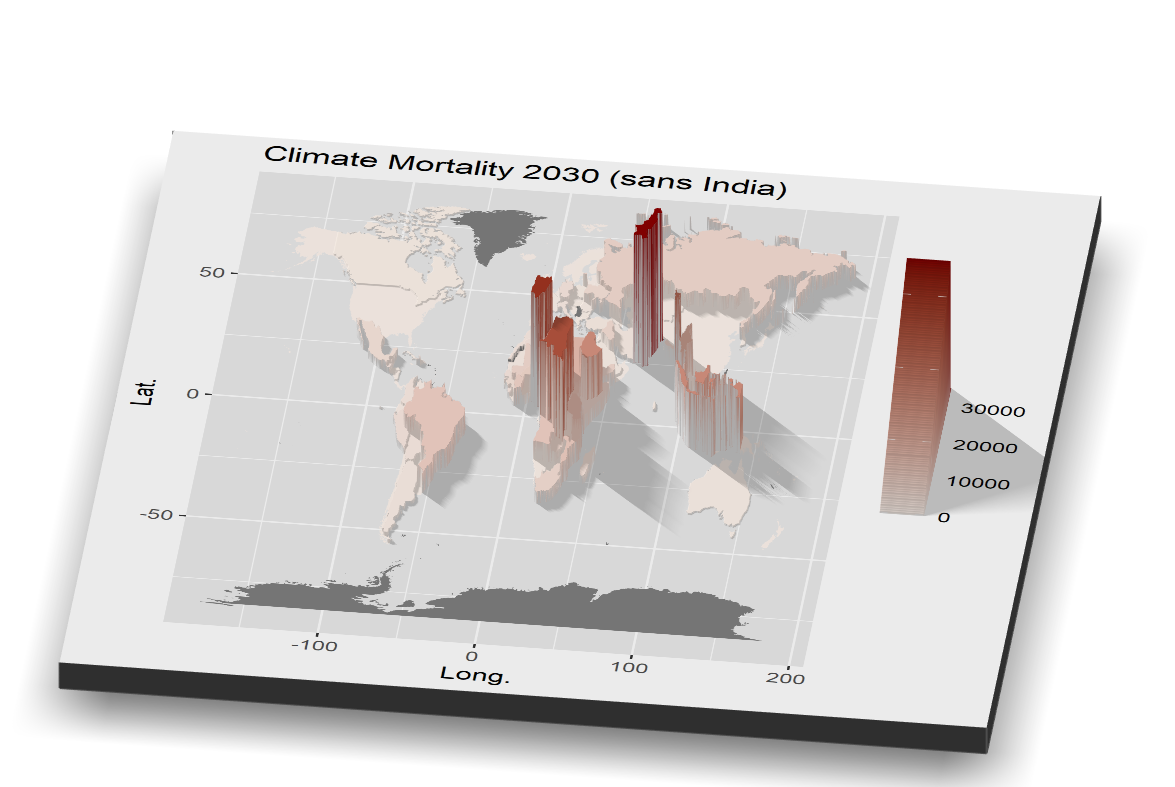
\includegraphics{Results/climmort_sansindia.png}
\caption{``Climate Mortality 2030 by Country (sans India)''}
\end{figure}

\end{document}
